\documentclass[11pt]{article}
\usepackage{../latex/colombiamacro}
\graphicspath{{../img/}{../figuras/}}

\title{ColombiaMacro}
\begin{document}

% ------------------------------------------------------------------ portada
\begin{titlepage}
\thispagestyle{empty}
\begin{tikzpicture}[remember picture,overlay]
  \fill[cmblue] (current page.north west) rectangle ([yshift=-9mm]current page.north east);
\end{tikzpicture}
\vspace*{18mm}
{\sffamily\small\color{cmmuted}UNIVERSIDAD DE SAN BUENAVENTURA CALI · FINANZAS Y NEGOCIOS INTERNACIONALES\par}
\vspace{16mm}
{\sffamily\bfseries\fontsize{38}{42}\selectfont ColombiaMacro\par}
\vspace{4mm}
{\Large Monitor del ciclo económico colombiano\par}
\vspace{10mm}
{\sffamily\LARGE\color{cmblue} Manual técnico y guía de lectura\par}
\vspace{6mm}
{\large Datos, métodos, presentación, operación y despliegue\par}
\vfill
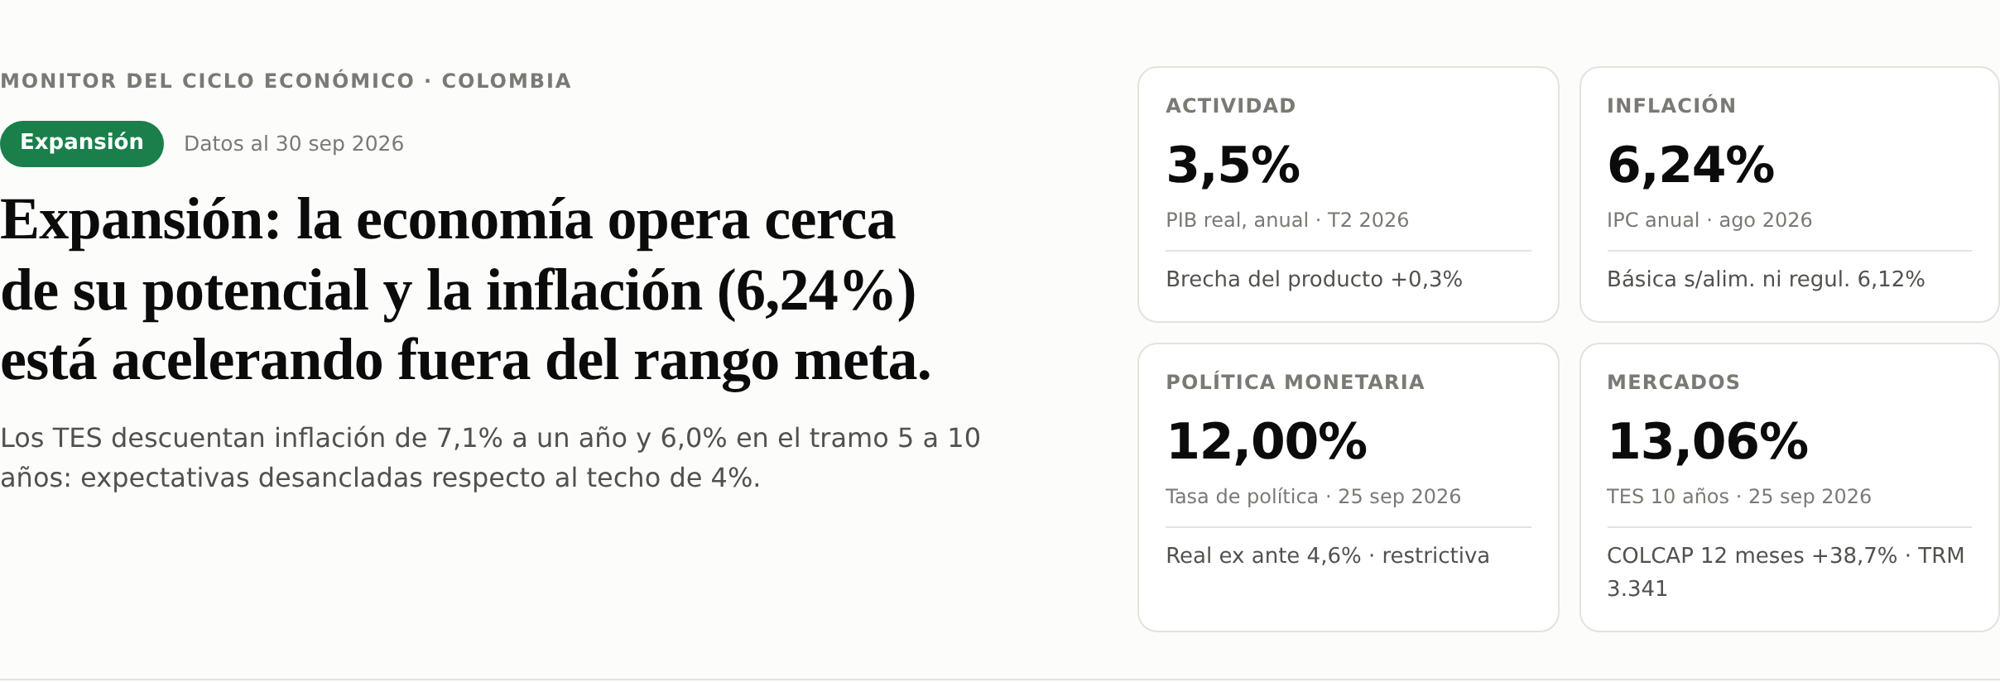
\includegraphics[width=\linewidth]{hero_es.png}
\vfill
\begin{tabularx}{\linewidth}{@{}Xr@{}}
{\sffamily\small Versión 9.0 · septiembre de 2026} & {\sffamily\small github.com/Stv-Quant/ColombiaMacro-USBCali}\\
\end{tabularx}
\end{titlepage}

\tableofcontents
\newpage

% ================================================================== 1
\section{Introducción}

\subsection{Qué es ColombiaMacro}
ColombiaMacro es un tablero web, abierto y reproducible, que responde una sola pregunta con
datos oficiales actualizados a diario:

\begin{center}
\sffamily\large ¿En qué fase del ciclo está la economía colombiana\\y qué implica para precios, política monetaria y activos?
\end{center}

La pregunta se descompone en cinco preguntas encadenadas, una por sección del tablero. El
orden no es casual: sigue la secuencia causal con la que un banco central lee la economía
(actividad $\rightarrow$ precios $\rightarrow$ reacción de política $\rightarrow$ precios de activos).

\begin{center}
\begin{tabularx}{\linewidth}{@{}lXX@{}}
\toprule
\textbf{Sección} & \textbf{Pregunta} & \textbf{Indicador principal}\\
\midrule
1. Actividad & ¿Crece la economía por encima de su potencial? & Brecha del producto (HP en tiempo real)\\
2. Precios & ¿Converge la inflación a la meta? & IPC total y básica; inflación implícita en TES\\
3. Política y curva & ¿Cuál es la postura de BanRep y qué descuenta el mercado? & Tasa real ex ante frente a la neutral\\
4. Mercados y externo & ¿Cómo lo reflejan la bolsa, el peso y las cuentas externas? & COLCAP (COP y USD), TRM, ITCR, cuenta corriente\\
5. Señales & ¿Qué tan extremo es cada dato? & Percentil histórico desde 2010\\
\bottomrule
\end{tabularx}
\end{center}

\subsection{Para quién es}
\begin{itemize}
\item \textbf{Inversionistas extranjeros}: una lectura en inglés o español, con las cifras que
importan para una asignación en Colombia (tasas reales, expectativas de inflación, peso, bolsa en dólares).
\item \textbf{Inversionistas y analistas locales}: un tablero diario con la misma disciplina metodológica
de un informe de banco central.
\item \textbf{Comunidad académica}: todas las fórmulas son explícitas, están probadas y se pueden reproducir
con un solo comando.
\end{itemize}

\subsection{Principios de diseño}
\begin{enumerate}
\item \textbf{Solo datos oficiales}: DANE, Banco de la República (BanRep), BVC/MSCI a través de BanRep y
Ministerio de Hacienda a través de BanRep. Nada se digita a mano.
\item \textbf{Identidad verificada}: cada serie se valida por número \emph{y} por nombre; si la fuente
reasigna un número, el proceso falla en lugar de publicar otra variable.
\item \textbf{Un eje, una unidad}: ningún gráfico tiene dos escalas verticales.
\item \textbf{Frases con respaldo}: el veredicto automático se deriva de reglas explícitas (sección~\ref{sec:veredicto}) y cita el dato que lo sustenta.
\item \textbf{Incertidumbre visible}: la brecha del producto se muestra como banda entre métodos, no como una sola cifra.
\item \textbf{Sin información futura}: los indicadores en tiempo real solo usan lo que se conocía en cada fecha.
\end{enumerate}

\subsection{Qué no es}
\begin{alerta}
No es una recomendación de inversión ni un pronóstico. La brecha del producto, la tasa neutral y las
expectativas implícitas son \emph{estimaciones} con incertidumbre documentada (sección~\ref{sec:limitaciones}).
\end{alerta}

% ================================================================== 2
\section{Recorrido rápido: el tablero en cinco minutos}
\label{sec:recorrido}

\captura[1]{topbar.png}{Barra superior: horizonte temporal (3, 5, 10 años o toda la historia) e idioma.}

\textbf{1. La barra superior.} El selector \emph{Horizonte} recorta todos los gráficos de series de tiempo
a la misma ventana; \emph{ES/EN} cambia todos los textos, incluidos el veredicto y los rótulos.

\textbf{2. El veredicto} (figura~\ref{fig:hero}). En una frase: la fase del ciclo (etiqueta de color),
la posición frente al potencial y la dirección de la inflación. Debajo, qué descuenta el mercado. A la
derecha, cuatro tarjetas con la cifra más importante de cada bloque y su fecha de referencia.

\begin{figure}[htbp]\centering
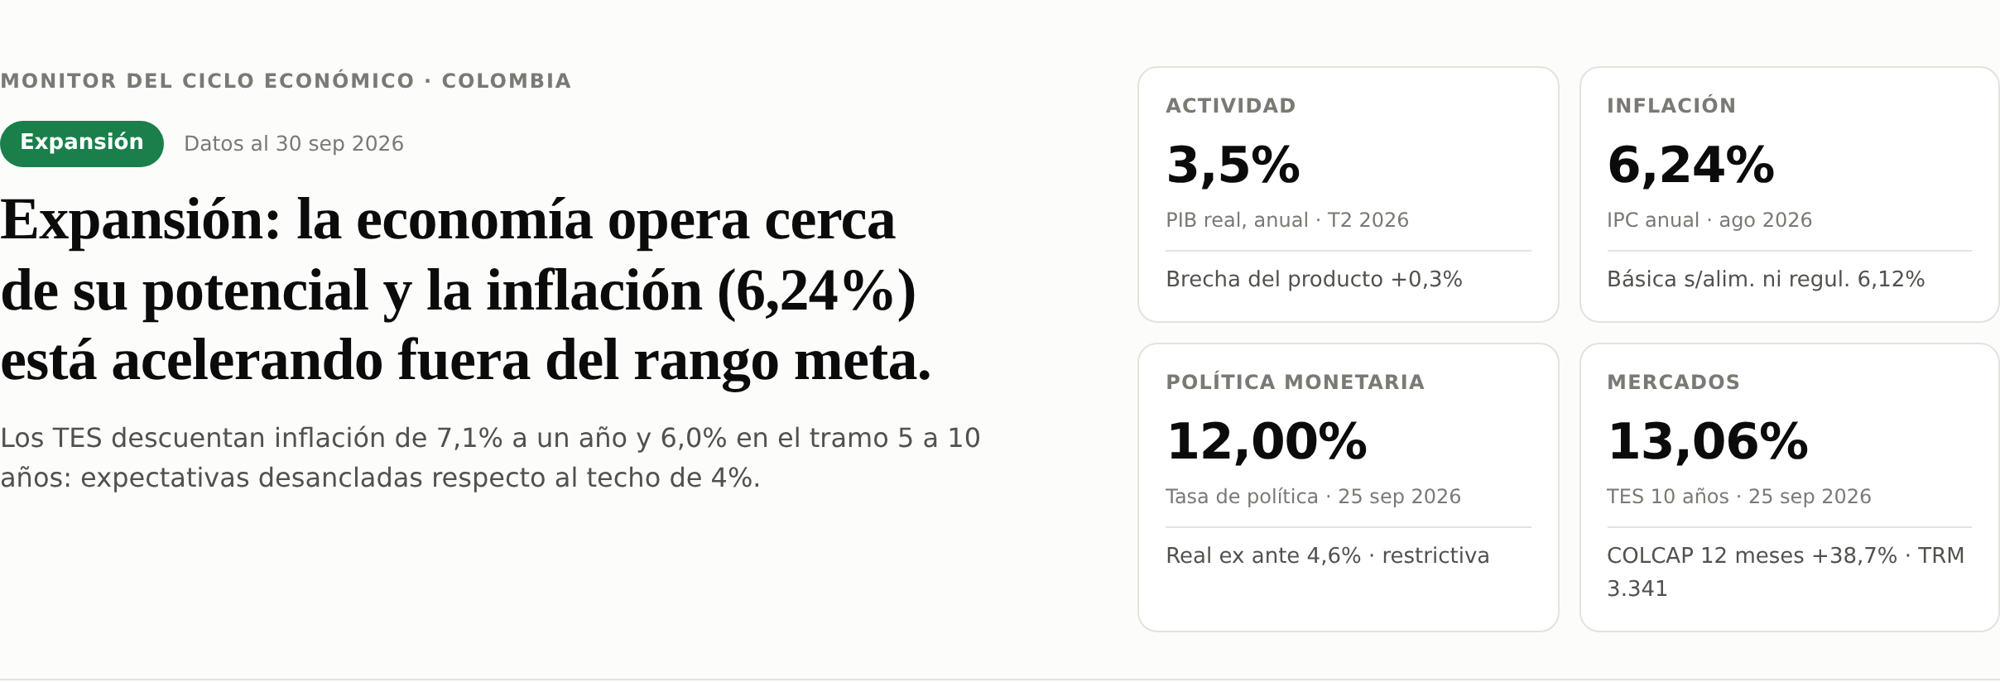
\includegraphics[width=\linewidth]{hero_es.png}
\caption{Veredicto y tarjetas principales (vista en español).}\label{fig:hero}
\end{figure}

\textbf{3. El índice de secciones} permite saltar a cada pregunta.

\textbf{4. Cada sección} empieza con un número, la pregunta, un párrafo de lectura generado a partir de
los datos, los gráficos y un desplegable \emph{Método y lectura} con las fórmulas.

\textbf{5. El tablero de señales} resume 16 indicadores con su último dato, cambio y percentil histórico.

\textbf{6. Al final}: el laboratorio (canastas bursátiles heredadas), el estado de cada fuente y los enlaces
para descargar todos los datos en CSV.

\begin{leer}[Regla de oro]
Lea siempre la \emph{fecha de referencia} junto a la cifra. El PIB es trimestral y se publica unos 45 días
después del trimestre; el IPC es mensual y se publica en la primera semana del mes siguiente; las tasas y
la bolsa son diarias. El tablero nunca rellena una frecuencia con otra.
\end{leer}

% ================================================================== 3
\section{Arquitectura del sistema}

\begin{figure}[htbp]\centering
\begin{tikzpicture}[
  box/.style={draw=cmrule,fill=white,rounded corners=2pt,align=center,font=\sffamily\scriptsize,minimum height=10mm,text width=29mm,inner sep=3pt},
  src/.style={box,fill=cmsoft},
  arr/.style={-{Stealth[length=2mm]},color=cmmuted,thick}]
\node[src] (dane) at (0,0.9) {DANE\\PIB · IPC · ISE · GEIH};
\node[src] (banrep) at (0,-0.9) {BanRep\\TES · COLCAP · TPM · TRM\\básica · sector externo};
\node[box] (upd) at (3.9,0) {Actualizadores\\\texttt{actualizar\_*.py}\\\texttt{banrep\_client.py}};
\node[box] (csv) at (7.8,0) {Tablas CSV\\versionadas en Git};
\node[box] (val) at (7.8,-1.9) {\texttt{validar\_datos.py}\\+ 43 pruebas};
\node[box] (app) at (11.7,0) {\texttt{analitica\_macro}\\\texttt{modelo\_tablero}\\\texttt{dashboard\_colombia}};
\node[box] (web) at (11.7,-1.9) {Servidor web\\Render / Docker};
\node[src] (user) at (11.7,-3.6) {Navegador ES / EN};
\draw[arr] (dane.east) -- (upd.west); \draw[arr] (banrep.east) -- (upd.west);
\draw[arr] (upd) -- (csv); \draw[arr] (csv) -- (val);
\draw[arr] (csv) -- (app); \draw[arr] (app) -- (web); \draw[arr] (web) -- (user);
\node[font=\sffamily\scriptsize,color=cmmuted,below=1mm of upd] {GitHub Actions · 19:30 diario};
\end{tikzpicture}
\caption{Flujo de datos. El servidor web nunca consulta las fuentes: solo lee CSV validados.}
\end{figure}

\subsection{Capas}
\begin{description}[style=nextline,leftmargin=0pt]
\item[Captura] \archivo{actualizar\_pib.py}, \archivo{actualizar\_inflacion.py}, \archivo{actualizar\_tes.py},
\archivo{actualizar\_colcap.py} y \archivo{actualizar\_macro\_extra.py} descargan cada fuente. Todas las
series de BanRep pasan por \archivo{banrep\_client.py}.
\item[Validación] \archivo{validar\_datos.py} recalcula fórmulas, revisa fechas, rangos y saltos, y escribe
\archivo{estado\_fuentes.csv} y \archivo{alertas\_datos.csv}.
\item[Analítica] \archivo{analitica\_macro.py} contiene funciones puras (entra una tabla, sale una tabla):
Fisher, inflación implícita, filtro HP, Hamilton, reloj del ciclo, percentiles.
\item[Modelo] \archivo{modelo\_tablero.py} carga todo, calcula la instantánea del último dato, redacta el
veredicto y arma la tabla de señales. Es la única fuente de cada cifra que aparece en pantalla.
\item[Presentación] \archivo{dashboard\_colombia.py} dibuja (Dash + Plotly). No calcula nada propio.
\end{description}

\subsection{Mapa de archivos}
\begin{longtable}{@{}p{0.36\linewidth}p{0.58\linewidth}@{}}
\toprule
\textbf{Archivo} & \textbf{Función}\\\midrule\endhead
\archivo{dashboard\_colombia.py} & Aplicación Dash v9; expone \texttt{server} para Gunicorn.\\
\archivo{modelo\_tablero.py} & Carga, instantánea, veredicto, tabla de señales; parámetros \texttt{NEUTRAL\_REAL}, umbrales.\\
\archivo{analitica\_macro.py} & Fórmulas y filtros.\\
\archivo{banrep\_client.py} & Cliente BanRep con cadena TLS completa.\\
\archivo{actualizar\_todo.py} & Orquestador de todas las fuentes.\\
\archivo{actualizar\_macro\_extra.py} & 16 series BanRep + ISE + GEIH.\\
\archivo{validar\_datos.py} & Controles de calidad y estado de fuentes.\\
\archivo{lanzar\_local.py} & Lanzador local con búsqueda de puerto libre.\\
\archivo{Iniciar ColombiaMacro.bat} & Doble clic en Windows.\\
\archivo{dashboard\_legacy.py} & Tablero anterior (v8), conservado para comparación.\\
\archivo{docs/generar\_figuras.py} & Figuras vectoriales para documentos y diapositivas.\\
\archivo{METODOLOGIA.md} & Nota metodológica breve.\\
\archivo{.github/workflows/actualizar-datos.yml} & Automatización diaria.\\
\archivo{render.yaml}, \archivo{Dockerfile} & Despliegue.\\
\archivo{tests/} & 43 pruebas unitarias e integradas.\\
\bottomrule
\end{longtable}

% ================================================================== 4
\section{Ejecución local}

\subsection{Requisitos}
Python 3.10 o superior (en Windows, marcar \emph{Add python.exe to PATH} al instalar) y conexión a internet
la primera vez (para instalar dependencias). No se requieren claves ni cuentas.

\subsection{Con doble clic (Windows)}
Abra la carpeta del proyecto y haga doble clic en \archivo{Iniciar ColombiaMacro.bat}. El lanzador:
\begin{enumerate}
\item crea el entorno virtual \archivo{.venv} la primera vez (unos 1–3 minutos);
\item instala o actualiza dependencias \emph{solo} si cambiaron los archivos \archivo{requirements};
\item busca un puerto libre empezando en 8050, \textbf{omitiendo 8765 y 8766} y cualquier puerto ocupado
(comprueba IPv4 e IPv6 e intenta reservarlo);
\item levanta el servidor \emph{waitress} en \texttt{127.0.0.1} (solo accesible desde su computador);
\item abre el navegador cuando el tablero responde.
\end{enumerate}

\begin{lstlisting}
[ColombiaMacro] Puertos omitidos (ocupados o reservados): 8050
[ColombiaMacro] Puerto elegido: 8051
[ColombiaMacro] Servidor waitress en http://127.0.0.1:8051/
[ColombiaMacro] Tablero listo en http://127.0.0.1:8051/  (Ctrl+C para detener)
\end{lstlisting}

\subsection{Opciones}
\begin{lstlisting}
python lanzar_local.py --puerto 8090          # preferir un puerto
python lanzar_local.py --evitar 8765 8766 3000 # puertos reservados adicionales
python lanzar_local.py --actualizar           # descarga DANE/BanRep antes de abrir
python lanzar_local.py --legacy               # tablero v8
python lanzar_local.py --solo-puerto          # solo informa el puerto
python lanzar_local.py --sin-navegador
\end{lstlisting}
En macOS o Linux: \texttt{./iniciar\_colombiamacro.sh} con las mismas opciones.

\begin{alerta}[Puertos]
Si otras aplicaciones locales se lanzan \emph{después} de ColombiaMacro y piden 8050, serán ellas las que
encuentren el puerto ocupado. Para fijar un rango lejano use \texttt{--puerto 8200}.
\end{alerta}

\subsection{Ejecutable .exe (opcional)}
Un archivo \texttt{.bat} ya se ejecuta con doble clic. Si necesita un \texttt{.exe} autónomo para
un equipo sin Python, en Windows:
\begin{lstlisting}
py -m pip install pyinstaller
py -m PyInstaller --onefile --name ColombiaMacro lanzar_local.py
\end{lstlisting}
El ejecutable resultante sigue necesitando la carpeta del proyecto (datos y código) al lado.

% ================================================================== 5
\section{Los datos}
\label{sec:datos}

Esta sección describe cada fuente: qué mide, cómo se obtiene, en qué unidad y con qué rezago.
La fecha de cada fila es el \emph{período medido}, no el día de publicación.

\subsection{Calendario y rezagos típicos}
\begin{center}\small
\begin{tabularx}{\linewidth}{@{}lllX@{}}
\toprule
\textbf{Variable} & \textbf{Frecuencia} & \textbf{Publicación} & \textbf{Implicación}\\\midrule
PIB (DANE) & Trimestral & $\approx$45 días después & El dato de T2 llega a mediados de agosto.\\
ISE (DANE) & Mensual & $\approx$50 días después & Adelanta el PIB del trimestre en curso.\\
IPC (DANE) & Mensual & 5–8 días después & El IPC de agosto se conoce en la primera semana de septiembre.\\
Desempleo GEIH & Mensual & $\approx$30 días después & Serie desestacionalizada del DANE.\\
TES, COLCAP, TRM, TPM & Diaria & Mismo día o siguiente & Base de la lectura de mercado.\\
Cuenta corriente & Trimestral & $\approx$75 días después & Rezago largo; leer tendencia.\\
Deuda del GNC & Anual & Varios meses & Contexto estructural.\\
\bottomrule
\end{tabularx}
\end{center}

\subsection{PIB real y nominal (DANE)}
\textbf{Archivo:} \archivo{pib\_colombia.csv}. \textbf{Origen:} anexos trimestrales del PIB por el enfoque
de la producción; Cuadro~1 (serie original) y Cuadro~4 (desestacionalizada y corregida por calendario),
volumen encadenado con referencia 2015; y el anexo a precios corrientes.
\begin{itemize}
\item \texttt{pib\_real\_yoy} $=100\,(Y_t/Y_{t-4}-1)$ con la serie original: crecimiento anual.
\item \texttt{pib\_real\_qoq\_sa} $=100\,(Y^{sa}_t/Y^{sa}_{t-1}-1)$: crecimiento trimestral desestacionalizado.
\item \texttt{pib\_nominal\_billones\_cop}: valor corriente, solo como magnitud.
\end{itemize}
\begin{dato}
T2 2026: crecimiento anual real 3,52\% (DANE redondea a 3,5\%). Nivel desestacionalizado 262.062 miles de
millones de pesos de 2015, frente a 258.732 en T1: crecimiento trimestral de 1,29\% (5,25\% anualizado).
\end{dato}
\begin{alerta}[Error corregido en la versión anterior]
Hasta la v7 el tablero mostraba como “crecimiento del PIB” la variación del PIB \emph{nominal}
(por eso aparecían 61\% en 2021). Desde la v8 se usa el volumen real encadenado.
\end{alerta}

\subsection{Índice de precios al consumidor (DANE y BanRep)}
\textbf{Archivo:} \archivo{inflacion\_clean.csv}. Índice de BanRep (serie 15000, base dic-2018=100) y las
variaciones que publica el DANE.
\begin{itemize}
\item \texttt{inflacion\_anual} $=100\,(IPC_t/IPC_{t-12}-1)$; el último mes se reemplaza por la cifra oficial
del DANE, porque el índice tiene dos decimales y el cálculo puede diferir 0,01~pp.
\item \texttt{inflacion\_mensual}: variación mensual reportada por el DANE.
\item Control: la inflación mensual compuesta en 12 meses reproduce la anual con error máximo 0,04~pp.
\end{itemize}

\subsection{Curvas cero cupón TES (BanRep)}
\textbf{Archivo:} \archivo{tasas\_interes\_clean.csv}. Series 15272–15274 (pesos, 1, 5 y 10 años) y
15275–15277 (UVR, mismos plazos). Son tasas efectivas anuales de la curva cero cupón estimada por BanRep
(modelo Nelson–Siegel), no rendimientos de un bono individual. Los TES UVR pagan un rendimiento
\emph{real}: su principal se indexa a la UVR, que sigue al IPC.

\subsection{COLCAP (BanRep, fuente BVC/MSCI)}
\textbf{Archivo:} \archivo{colcap\_oficial.csv}, serie 6. \texttt{colcap\_base100} $=100\,P_t/P_{9\text{-feb-}2009}$.
El 28 de mayo de 2021 el índice pasó de la metodología BVC a MSCI COLCAP, con continuidad de niveles: la
serie es numéricamente continua, pero la canasta y las ponderaciones cambiaron. El gráfico marca esa fecha.

\subsection{Series complementarias BanRep}
\textbf{Archivo:} \archivo{series\_banrep.csv}, formato largo \texttt{(fecha, serie, valor, frecuencia, unidad, id\_banrep)}.
Las fechas mensuales se normalizan al primer día del mes; las trimestrales, al primer día del trimestre;
las anuales, al 1 de enero. Se descartan períodos que aún no comienzan (la meta se publica por adelantado).

\begin{longtable}{@{}p{0.34\linewidth}rp{0.16\linewidth}p{0.3\linewidth}@{}}
\toprule
\textbf{Serie} & \textbf{Id} & \textbf{Unidad} & \textbf{Uso en el tablero}\\\midrule\endhead
Tasa de política monetaria & 59 & \% e.a. & Postura, tasa real, pendiente 10A–TPM\\
IBR overnight efectiva & 15324 & \% e.a. & Referencia del mercado monetario\\
TRM & 1 & COP/USD & COLCAP en dólares, gráfico de tasa de cambio\\
Inflación sin alimentos & 15388 & \% anual & Básica\\
Inflación sin alimentos ni regulados & 15390 & \% anual & Básica principal\\
Inflación núcleo 15 & 15392 & \% anual & Básica alternativa\\
Inflación de regulados & 15398 & \% anual & Componentes\\
Inflación de alimentos & 15404 & \% anual & Componentes\\
Meta de inflación & 853 & \% & Historia de la meta\\
ITCR-IPC ponderaciones totales & 235 & 2010=100 & Tasa de cambio real\\
Términos de intercambio & 15360 & índice & Contexto externo\\
Reservas internacionales netas & 15051 & USD mn & Contexto externo\\
Cuenta corriente & 15290 & \% PIB & Sector externo\\
IED en Colombia & 15133 & USD mn & Sector externo\\
Deuda bruta del GNC & 15328 & \% PIB & Fiscal\\
Salario mínimo, variación & 15418 & \% anual & Contexto de precios\\
\bottomrule
\end{longtable}

\subsection{ISE y mercado laboral (DANE)}
\textbf{ISE} (\archivo{ise\_mensual.csv}): anexo \emph{ISE 9 actividades}; Cuadro~1 (original) y Cuadro~2
(desestacionalizado), base 2015=100, total y grandes ramas (primarias, secundarias, terciarias).
\textbf{GEIH} (\archivo{mercado\_laboral.csv}): anexo desestacionalizado, total nacional: tasa global de
participación (TGP), tasa de ocupación (TO) y tasa de desocupación (TD). El validador comprueba la identidad
$TD = 100\,(1-TO/TGP)$.

\subsection{Tablas heredadas}
\archivo{indices\_colombia.csv}, \archivo{precios\_icolcap\_limpios.csv}, \archivo{Canasta\_Historica\_ICAP.xls}
e \archivo{indices\_experimentales\_mensuales.csv} alimentan solo el laboratorio de canastas
(sección~\ref{sec:lab}). No intervienen en ninguna cifra del tablero principal.

% ================================================================== 6
\section{Transformaciones y fórmulas}
\label{sec:formulas}

Cada fórmula está en \archivo{analitica\_macro.py} y tiene una prueba en \archivo{tests/}. Los ejemplos
usan los datos al 25 de septiembre de 2026.

\subsection{Identidad de Fisher exacta}
Toda conversión entre tasas nominales y reales usa la forma exacta
\[
1+i = (1+r)(1+\pi) \quad\Longrightarrow\quad r = \frac{1+i}{1+\pi}-1,
\]
y no la aproximación $r\approx i-\pi$, que con tasas de dos dígitos sesga el resultado en más de 0,3~pp.

\subsection{Inflación implícita (breakeven)}
Para un plazo $h$, con $i_h$ la tasa TES en pesos y $r_h$ la tasa TES UVR:
\[
\pi^{BE}_h = 100\left[\frac{1+i_h/100}{1+r_h/100}-1\right].
\]
\begin{dato}[Ejemplo]
A 1 año: $i_1=12{,}42\%$, $r_1=4{,}99\%$ $\Rightarrow$ $\pi^{BE}_1 = 100\,(1{,}1242/1{,}0499-1)=7{,}08\%$.
A 10 años: $13{,}06\%$ y $6{,}64\%$ $\Rightarrow$ $6{,}02\%$.
\end{dato}
La inflación implícita no es una expectativa pura: incluye una prima por riesgo inflacionario (el inversionista
exige compensación por la incertidumbre de la inflación) y una prima por liquidez (los TES UVR se negocian
menos). Por eso el tablero la describe como “lo que el mercado descuenta”.

\subsection{Forward 5y5y}
Mide la inflación promedio implícita entre los años 5 y 10, un horizonte en el que la política monetaria
debería haber llevado la inflación a la meta; es el indicador estándar de \emph{anclaje}.
\[
f^{nom}=\left(\frac{(1+i_{10})^{10}}{(1+i_5)^{5}}\right)^{1/5}\!-1,\qquad
f^{real}=\left(\frac{(1+r_{10})^{10}}{(1+r_5)^{5}}\right)^{1/5}\!-1,\qquad
\pi^{5y5y}=\frac{1+f^{nom}}{1+f^{real}}-1.
\]
\begin{dato}[Ejemplo]
$i_5=12{,}90$, $i_{10}=13{,}06$ $\Rightarrow f^{nom}=13{,}22\%$; $r_5=6{,}48$, $r_{10}=6{,}64$
$\Rightarrow f^{real}=6{,}80\%$; $\pi^{5y5y}=1{,}1322/1{,}0680-1=6{,}01\%$. Por encima del techo de 4\%:
expectativas \emph{desancladas}.
\end{dato}

\subsection{Tasa de política real}
\[
r^{ex\,ante}_t=\frac{1+TPM_t}{1+\pi^{BE}_{1,t}}-1,\qquad
r^{ex\,post}_t=\frac{1+TPM_t}{1+\pi^{obs}_{t}}-1 .
\]
$\pi^{obs}_t$ es la última inflación \emph{publicada} a la fecha $t$: el IPC del mes $m$ se considera disponible
el día 10 del mes $m+1$. Así el cálculo nunca usa un dato que aún no se conocía.
\begin{dato}[Ejemplo]
$TPM=12\%$, $\pi^{BE}_1=7{,}08\%$ $\Rightarrow r^{ex\,ante}=1{,}12/1{,}0708-1=4{,}60\%$ (la aproximación daría 4,92\%).
Con el IPC de agosto (6,24\%): $r^{ex\,post}=5{,}42\%$.
\end{dato}

\subsection{Brecha del producto}
Sea $y_t=100\ln Y^{sa}_t$ (PIB real desestacionalizado). La tendencia $\tau$ del filtro de Hodrick y Prescott
(1997) resuelve
\[
\min_{\{\tau_t\}}\ \sum_{t=1}^{T}(y_t-\tau_t)^2+\lambda\sum_{t=2}^{T-1}\big[(\tau_{t+1}-\tau_t)-(\tau_t-\tau_{t-1})\big]^2,
\qquad \lambda=1600,
\]
cuya solución matricial es $\tau=(I+\lambda D^\top D)^{-1}y$, con $D$ la matriz de segundas diferencias
de dimensión $(T-2)\times T$. La brecha es $g_t=y_t-\tau_t$, en porcentaje del producto potencial.

\subsubsection*{Por qué “en tiempo real”}
El filtro de dos colas usa observaciones futuras: la tendencia de 2019 cambia cuando llega el dato de 2021.
Orphanides y van Norden (2002) muestran que esas revisiones son del mismo orden que la brecha misma. La
estimación principal del tablero resuelve el problema para cada $t$ usando solo $y_1,\dots,y_t$ y conserva
el último punto $\tau_{t|t}$. Se exige un mínimo de 20 trimestres. La implementación coincide con
\texttt{statsmodels.hpfilter} hasta $2\times10^{-10}$.

\subsubsection*{Contrastes}
\begin{itemize}
\item \textbf{HP de dos colas} ($\tau_{t|T}$): mejor estimación ex post.
\item \textbf{Hamilton (2018)}: residuo de la regresión $y_{t+8}=\beta_0+\sum_{k=0}^{3}\beta_k\,y_{t-k}+v_{t+8}$ por MCO;
evita las propiedades espurias del HP en series integradas.
\end{itemize}

\subsubsection*{Tratamiento del COVID}
Los trimestres 2020-T2 a 2021-T2 se reemplazan por interpolación lineal \emph{solo para estimar la tendencia}
(y los coeficientes de Hamilton). La brecha se mide siempre contra el dato observado. Sin este tratamiento, una
caída de 17,6\% en un trimestre arrastra la tendencia y distorsiona la lectura de 2019–2023.

\subsubsection*{Crecimiento potencial}
$g^{pot}_t=100\,[\exp((\tau_t-\tau_{t-4})/100)-1]$ con la tendencia HP de dos colas. Al T2 2026: 2,37\%.

\subsection{Reloj del ciclo}
Con $\Delta_2 g_t=g_t-g_{t-2}$ (cambio en dos trimestres, para suavizar el ruido de un solo dato):
\begin{center}
\begin{tabular}{@{}lcc@{}}
\toprule
 & $\Delta_2 g_t\ge 0$ & $\Delta_2 g_t<0$\\\midrule
$g_t\ge 0$ & \textcolor{cmgreen}{\textbf{Expansión}} & \textcolor{cmamber}{\textbf{Desaceleración}}\\
$g_t<0$ & \textcolor{cmblue}{\textbf{Recuperación}} & \textcolor{cmred}{\textbf{Contracción}}\\
\bottomrule
\end{tabular}
\end{center}
Es la lógica del \emph{business cycle clock} de la OCDE.

\subsection{ISE: ritmo de corto plazo}
Variación anual con la serie original (comparable con el PIB) y ritmo trimestral anualizado con la
desestacionalizada: $100\,[(\bar{x}_{t,3}/\bar{x}_{t-3,3})^4-1]$, donde $\bar{x}_{t,3}$ es el promedio de los
últimos tres meses.

\subsection{Percentil histórico}
Para cada indicador, la proporción de observaciones desde 2010 menores o iguales al último dato.
Un percentil de 96 significa que el dato actual es mayor que el 96\% de su propia historia desde 2010.

\subsection{Retornos y COLCAP en dólares}
Retorno a 12 meses: último dato frente al último dato disponible 365 días antes.
COLCAP en dólares: puntos divididos por la TRM del mismo día (tolerancia de 7 días).

\subsection{Saltos aislados}
Una observación se considera salto aislado si se aleja más de $u$ de ambos vecinos mientras los vecinos
difieren menos de $v$: $|x_t-x_{t-1}|>u$, $|x_t-x_{t+1}|>u$, $|x_{t-1}-x_{t+1}|<v$. Para las tasas TES
$(u,v)=(2,1)$~pp; para las series derivadas $(1;\,0{,}5)$~pp. Los valores originales se conservan en los CSV;
solo se excluyen de los cálculos y se registran.

% ================================================================== 7
\section{Guía de lectura, gráfico por gráfico}
\label{sec:lectura}

\subsection{Sección 1 · Actividad}
\captura{lectura_1.png}{Párrafo de lectura de la sección de actividad.}

\subsubsection*{Brecha del producto}
\captura[0.8]{chart_01_brecha_del_producto_del_pib_potencial.png}{Brecha del producto: estimación principal y rango entre métodos.}
\begin{leer}
La línea azul es la estimación principal. La banda es el rango entre los tres métodos. Arriba de cero, la
economía produce más que su potencial (presión sobre precios); abajo, hay holgura. Una banda angosta indica
consenso entre métodos; una ancha, que la lectura depende del supuesto.
\end{leer}
\begin{alerta}[Error frecuente]
Confundir crecimiento con brecha. Una economía puede crecer 3,5\% y aun así estar \emph{cerca} del potencial si
viene de una brecha negativa. Lo relevante para la inflación es el \emph{nivel} de la brecha.
\end{alerta}

\subsubsection*{Reloj del ciclo}
\captura[0.8]{chart_02_reloj_del_ciclo_nivel_y_direccion_de_la_.png}{Reloj del ciclo: últimos doce trimestres.}
\begin{leer}
Cada punto es un trimestre; el grande es el último. El eje horizontal es el nivel de la brecha; el vertical,
su cambio en dos trimestres. El recorrido típico gira en sentido horario: recuperación $\rightarrow$
expansión $\rightarrow$ desaceleración $\rightarrow$ contracción.
\end{leer}

\subsubsection*{Crecimiento real anual}
\captura[0.8]{chart_03_crecimiento_real_anual_pib_trimestral_is.png}{PIB trimestral, ISE mensual y crecimiento potencial.}
\begin{leer}
El ISE adelanta el PIB del trimestre en curso. Cuando el crecimiento supera al potencial (línea punteada),
la brecha tiende a cerrarse o a volverse positiva. Los valores de 2020–2022 quedan fuera de escala para no
aplastar la lectura reciente; el tooltip los muestra.
\end{leer}

\subsubsection*{Desempleo}
Tasa de desocupación desestacionalizada (mensual y promedio de 3 meses). Un desempleo que cae mientras la
brecha es positiva refuerza la lectura de presión de demanda.

\subsection{Sección 2 · Precios}
\captura[0.8]{chart_05_inflacion_total_y_basica_frente_al_rango.png}{Inflación total y básica frente al rango meta.}
\begin{leer}
La franja verde es el rango meta de BanRep (3\% $\pm$ 1~pp). La básica (sin alimentos ni regulados) mide la
presión persistente; si la total sube pero la básica no, el choque es probablemente transitorio (alimentos,
tarifas). Hoy ambas están por encima de 6\%: la presión es generalizada.
\end{leer}

\captura[0.8]{chart_06_expectativas_de_mercado_inflacion_implic.png}{Inflación implícita en TES a 1 año y 5y5y.}
\begin{leer}
Si la 5y5y (morada) se mantiene dentro del rango, el mercado confía en que la inflación volverá a la meta
aunque hoy esté alta. Una 5y5y persistentemente por encima de 4\% indica expectativas desancladas: el
mercado duda de la convergencia y exige más prima en los bonos largos.
\end{leer}

\subsection{Sección 3 · Política monetaria y curva}
\captura[0.8]{chart_08_tasa_de_politica_frente_a_inflacion.png}{Tasa de política frente a inflación observada e implícita.}
\captura[0.8]{chart_09_tasa_de_politica_real_ex_ante_frente_a_l.png}{Tasa real ex ante y ex post frente a la neutral.}
\begin{leer}
La postura depende de la tasa \emph{real}, no de la nominal. Por encima de la banda gris (neutral estimada
2,7–3,0\%) la política frena la demanda; por debajo, la estimula. La ex ante (con la inflación que descuenta
el mercado) es la relevante para decisiones de inversión y consumo.
\end{leer}
\captura[0.7]{chart_10_curva_cero_cupon_tes_pesos.png}{Curva cero cupón TES pesos: hoy, hace 3 y hace 12 meses.}
\begin{leer}
La curva muestra cuánto rinde prestarle al Gobierno a 1, 5 y 10 años. Un desplazamiento hacia arriba de toda
la curva (como entre septiembre de 2025 y hoy) refleja una tasa de política más alta y mayores primas; una
curva plana o invertida suele anticipar recortes o menor crecimiento.
\end{leer}
\captura[0.8]{chart_11_pendiente_de_la_curva.png}{Pendientes 10A–1A y 10A–tasa de política.}

\subsection{Sección 4 · Mercados y sector externo}
\captura[0.8]{chart_12_colcap_en_pesos_y_en_dolares_base_100_al.png}{COLCAP en pesos y en dólares, base 100 al inicio del horizonte.}
\begin{leer}
Para un inversionista extranjero el retorno relevante es en dólares: combina el precio de las acciones y la
tasa de cambio. Si la línea en dólares supera a la de pesos, el peso se apreció en el período.
COLCAP es un índice de precios: no incluye dividendos.
\end{leer}
\captura[0.8]{chart_13_tasa_de_cambio_nominal_pesos_por_dolar_t.png}{TRM: pesos por dólar.}
\captura[0.8]{chart_14_tasa_de_cambio_real_multilateral_itcr_ip.png}{Tasa de cambio real multilateral.}
\begin{leer}
El ITCR compara precios de Colombia con los de sus socios comerciales, en una misma moneda. Por debajo de
100 el peso está más fuerte en términos reales que en 2010: las importaciones se abaratan y la
competitividad de las exportaciones no tradicionales se reduce.
\end{leer}
\captura[0.8]{chart_15_cuenta_corriente_del_pib_trimestral.png}{Cuenta corriente, porcentaje del PIB.}
\captura[0.8]{chart_16_deuda_bruta_del_gobierno_nacional_centra.png}{Deuda bruta del Gobierno Nacional Central.}

\subsection{Sección 5 · Tablero de señales}
\captura{senales.png}{Tablero de señales.}
\begin{leer}
Cada fila tiene el último dato, su fecha, el cambio (en pp para tasas y en \% para niveles como COLCAP o TRM)
y el percentil desde 2010. Las barras oscuras marcan valores extremos (percentil $\le 10$ o $\ge 90$): son
los datos que más se alejan de su normalidad histórica y merecen atención.
\end{leer}

\subsection{Laboratorio de canastas}
\label{sec:lab}
\captura[0.85]{chart_lab.png}{Laboratorio: COLCAP oficial frente a reconstrucciones heredadas.}
Las curvas “equiponderada” y “7 Magníficas” son reconstrucciones del proyecto original: retornos mensuales de
canastas locales distribuidos a días, sin ajuste por dividendos ni eventos corporativos y con composición
posterior a 2021 aproximada. Se conservan para revisión metodológica; no son índices oficiales.

% ================================================================== 8
\section{El veredicto automático}
\label{sec:veredicto}

Todas las frases salen de \archivo{modelo\_tablero.veredicto()} con estas reglas:
\begin{center}\small
\begin{tabularx}{\linewidth}{@{}lXl@{}}
\toprule
\textbf{Concepto} & \textbf{Regla} & \textbf{Parámetro}\\\midrule
Fase & Cuadrante del reloj del ciclo con la brecha HP en tiempo real & —\\
Frente al potencial & cerca si $|g|<0{,}5$; encima si $g\ge0{,}5$; debajo si $g\le-0{,}5$ & \texttt{UMBRAL\_BRECHA}\\
Dirección de la inflación & acelera si el cambio de 3 meses $>0{,}1$~pp; cede si $<-0{,}1$~pp & —\\
Fuera del rango & inflación $>4\%$ o $<2\%$ & —\\
Postura & restrictiva si $r^{ex\,ante}>3{,}0+0{,}5$; expansiva si $<2{,}7-0{,}5$ & \texttt{NEUTRAL\_REAL}, \texttt{UMBRAL\_POSTURA}\\
Anclaje & desancladas si 5y5y $>4\%$ & \texttt{ANCLA\_EXPECTATIVAS}\\
\bottomrule
\end{tabularx}
\end{center}

\begin{dato}[Veredicto al corte]
\emph{“Expansión: la economía opera cerca de su potencial y la inflación (6,24\%) está acelerando fuera del
rango meta.”} Brecha $+0{,}3\%$ (rango $+0{,}3$ a $+2{,}3$); IPC $+0{,}40$~pp en tres meses; tasa real ex ante
4,6\% (restrictiva); 5y5y 6,0\% (desancladas).
\end{dato}

Los parámetros están al inicio de \archivo{modelo\_tablero.py}. Cambiarlos modifica la redacción
automáticamente; las pruebas verifican que las frases citen las cifras correctas.

% ================================================================== 9
\section{Control de calidad y validación}

\subsection{Controles automáticos}
\begin{itemize}
\item Identidad de cada serie por número y nombre (insensible a tildes).
\item Rangos plausibles por serie; historia mínima (1000 días, 60 meses, 40 trimestres, 10 años).
\item Fechas sin duplicados, sin futuros, sin meses o trimestres faltantes.
\item Recalculo de fórmulas en cada corrida: PIB (tres tasas), IPC, ISE, identidad de la GEIH, COLCAP base 100.
\item Saltos aislados listados en \archivo{alertas\_datos.csv}.
\item 43 pruebas: fórmulas (Fisher, 5y5y, HP frente a una serie lineal, ausencia de información futura en el
HP en tiempo real, Hamilton en una caminata con deriva), cliente BanRep, lectores DANE, tablero completo
en ambos idiomas y tres horizontes, lista blanca de descargas.
\end{itemize}

\subsection{Robustez de la brecha del producto}
\begin{center}\small
\begin{tabular}{@{}lr@{}}
\toprule
\textbf{Métrica (51 trimestres, 2013-T4 a 2026-T2)} & \textbf{Valor}\\\midrule
Coincidencia de signo: HP tiempo real vs. HP dos colas & 78\%\\
Coincidencia de signo: HP tiempo real vs. Hamilton & 65\%\\
Coincidencia de fase: HP tiempo real vs. Hamilton & 43\%\\
Revisión media, tiempo real menos dos colas & $-0{,}52$~pp (MAE 0,96)\\
Correlación entre métodos sin 2020–21 & 0,66–0,77\\
\bottomrule
\end{tabular}
\end{center}
\captura[0.9]{brecha_producto.pdf}{Brecha del producto con los tres métodos (figura vectorial).}

\subsection{Validación de la inflación implícita}
\begin{center}\small
\begin{tabular}{@{}lrrrr@{}}
\toprule
\textbf{Período} & \textbf{Meses} & \textbf{Sesgo} & \textbf{RMSE implícita} & \textbf{RMSE caminata aleatoria}\\\midrule
2006–2019 & 168 & $+0{,}48$ & 1,70 & 2,08\\
2020–2025 & 68 & $+2{,}32$ & 4,13 & 4,07\\
Total & 236 & $+1{,}01$ & 2,64 & 2,80\\
\bottomrule
\end{tabular}
\end{center}
Sesgo = inflación realizada 12 meses después menos implícita a 1 año (pp). Antes de 2020 la implícita
pronostica mejor que suponer que la inflación no cambia; el choque 2021–23 no lo anticipó ningún método.
\captura[0.6]{validacion_bei.pdf}{Implícita a 1 año frente a la inflación realizada 12 meses después.}

% ================================================================== 10
\section{Automatización y operación}

\subsection{Flujo diario}
El workflow \archivo{.github/workflows/actualizar-datos.yml} corre todos los días a las 00:30 UTC (19:30
Colombia) y también a demanda (\emph{Run workflow}):
\begin{enumerate}
\item instala dependencias y corre las pruebas;
\item ejecuta \archivo{actualizar\_todo.py} (si una fuente falla, las demás continúan);
\item valida las tablas y corre de nuevo las pruebas con los datos nuevos;
\item publica un commit solo si los CSV cambiaron;
\item marca el run como fallido si alguna fuente falló, para que llegue una alerta por correo.
\end{enumerate}
El servidor web se redespliega al recibir el commit (auto-deploy).

\subsection{Estado de las fuentes}
\archivo{estado\_fuentes.csv} lista cada fuente con su último período y uno de tres estados:
\emph{vigente}, \emph{rezagado} (supera el umbral de días esperado) o \emph{pendiente} (aún no descargada).
Se ve en el desplegable \emph{Fuentes, vigencia y descargas}.

\subsection{Primera carga tras publicar el repositorio}
\begin{enumerate}
\item En GitHub: \emph{Settings $\rightarrow$ Actions $\rightarrow$ General $\rightarrow$ Workflow permissions}: \emph{Read and write}.
\item \emph{Actions $\rightarrow$ Actualizar indicadores Colombia $\rightarrow$ Run workflow}.
\item Verificar que aparezca un commit “Actualizar indicadores publicados” con \archivo{series\_banrep.csv},
\archivo{ise\_mensual.csv} y \archivo{mercado\_laboral.csv}.
\end{enumerate}

\subsection{El caso del certificado de BanRep}
El servidor \texttt{suameca.banrep.gov.co} envía su certificado sin el intermedio \emph{GeoTrust EV RSA CA G2}.
Los navegadores lo completan solos; Python en Linux no. \archivo{banrep\_client.py} agrega ese intermedio
(versionado en \archivo{certs/}) a las raíces de confianza, sin desactivar la verificación TLS. Antes de la v9
solo el actualizador de TES lo hacía, y por eso el COLCAP dejó de actualizarse el 24 de septiembre de 2026.

% ================================================================== 11
\section{Despliegue}
\label{sec:deploy}

\begin{center}\small
\begin{tabularx}{\linewidth}{@{}lXX@{}}
\toprule
\textbf{Opción} & \textbf{Ventajas} & \textbf{Limitaciones}\\\midrule
Render (plan free) & Ya configurado (\archivo{render.yaml}); auto-deploy desde GitHub & Se suspende tras 15 min sin tráfico; tarda cerca de un minuto en despertar\\
Render (plan starter) & Siempre activo, mismo flujo; recomendado para presentaciones & Costo mensual (del orden de 7 USD)\\
Google Cloud Run (Docker) & Escala a cero, HTTPS, dominio propio; instancia mínima para evitar arranques en frío & Requiere cuenta GCP y facturación\\
Servidor de la universidad (Docker) & Dominio institucional (p. ej. \texttt{colombiamacro.usbcali.edu.co}), control de TI & Depende de la oficina de TI; actualizar con \texttt{git pull} programado\\
Hugging Face Spaces (Docker) & Gratuito, visibilidad académica & Se suspende por inactividad; no institucional\\
\bottomrule
\end{tabularx}
\end{center}

\textbf{Recomendación}: Render con el repositorio nuevo, plan \emph{starter} durante el período de
presentaciones (sin arranques en frío), y el \archivo{Dockerfile} como ruta para migrar a un servidor
institucional de la universidad. Siempre llevar la versión local como respaldo.

\subsection{Render paso a paso}
\begin{enumerate}
\item En Render: \emph{New $\rightarrow$ Blueprint} y elegir el repositorio \texttt{ColombiaMacro-USBCali}.
\item Render lee \archivo{render.yaml}: servicio \texttt{colombiamacro-usbcali}, Python 3.12, Gunicorn.
\item Cambiar el plan a \emph{Starter} si se requiere disponibilidad permanente.
\item Verificar \emph{Auto-Deploy: Yes} para que cada commit de datos redepliegue.
\end{enumerate}

\subsection{Docker}
\begin{lstlisting}
docker build -t colombiamacro .
docker run -p 8080:8080 colombiamacro     # http://localhost:8080
\end{lstlisting}

% ================================================================== 12
\section{Mantenimiento y extensión}

\subsection{Agregar una serie de BanRep}
\begin{enumerate}
\item Encontrar el número en el graficador de BanRep
(\url{https://suameca.banrep.gov.co/graficador-series/}); la URL de consulta es
\texttt{.../consultaSerieParaGraficar?idSerie=N}.
\item Agregar una entrada en \texttt{SERIES} de \archivo{actualizar\_macro\_extra.py}:
\begin{lstlisting}[language=Python]
"embi_colombia": (NNNN, "texto del nombre", "diaria", "pb", (0, 2000)),
\end{lstlisting}
\item Agregarla a la lista de \texttt{extra} en \archivo{modelo\_tablero.cargar()} y, si debe vigilarse, a
\texttt{BANREP\_SERIES} en \archivo{validar\_datos.py}.
\item Crear su gráfico en \archivo{dashboard\_colombia.py} con \texttt{base\_fig} y \texttt{line}.
\item Correr \texttt{python -m unittest discover -s tests}.
\end{enumerate}

\subsection{Cambiar parámetros metodológicos}
\texttt{NEUTRAL\_REAL}, \texttt{UMBRAL\_BRECHA}, \texttt{UMBRAL\_POSTURA} y \texttt{ANCLA\_EXPECTATIVAS} en
\archivo{modelo\_tablero.py}; \texttt{HP\_LAMBDA\_TRIMESTRAL}, \texttt{HAMILTON\_H}, \texttt{HAMILTON\_P} y la ventana
COVID en \archivo{analitica\_macro.py}. Documentar todo cambio en \archivo{METODOLOGIA.md}.

\subsection{Regenerar figuras de documentos}
\begin{lstlisting}
python docs/generar_figuras.py     # docs/figuras/*.pdf, *.png y resumen.json
\end{lstlisting}

% ================================================================== 13
\section{Limitaciones}
\label{sec:limitaciones}
\begin{enumerate}
\item \textbf{Una sola vintage}: las cifras históricas son las de la última publicación, no lo que se sabía en
cada fecha. La brecha en tiempo real elimina la información futura del filtro, pero no las revisiones del DANE.
\item \textbf{La fase depende del método} (coincidencia de fase de 43\% entre HP en tiempo real y Hamilton).
\item \textbf{La tasa neutral es externa} y tiene incertidumbre amplia.
\item \textbf{Las implícitas contienen primas} variables en el tiempo.
\item \textbf{COLCAP no mide retorno total} (sin dividendos).
\item \textbf{Canastas heredadas}: sin ajuste por eventos corporativos ni composición histórica completa.
\end{enumerate}

\subsection*{Trabajo futuro}
Base de datos de vintages (real-time dataset) del PIB; modelo de factores dinámicos con indicadores mensuales
para estimar la brecha (nowcasting); descomposición de la implícita en expectativa y prima con un modelo afín
de la curva; riesgo país (CDS/EMBI) si se obtiene una fuente con derechos de redistribución.

% ================================================================== 14
\section{Solución de problemas}
\begin{description}[style=nextline,leftmargin=0pt]
\item[“No se encontró Python”] Instalar Python 3.10+ desde python.org marcando \emph{Add python.exe to PATH}.
\item[El navegador no abre] Copiar la URL que muestra la consola (\texttt{http://127.0.0.1:PUERTO/}).
\item[Otro programa usa el puerto] El lanzador lo detecta y elige otro; para reservar más: \texttt{--evitar}.
\item[Sección “pendiente de primera descarga”] Ejecutar el workflow manualmente o \texttt{--actualizar} en local.
\item[Fuente “rezagada”] Revisar el run de GitHub Actions; si la fuente cambió de formato, el mensaje de error
indica la serie y la causa.
\item[\texttt{CERTIFICATE\_VERIFY\_FAILED} con BanRep] Verificar que \archivo{certs/GeoTrustEVRSACAG2.pem} exista
y que el código use \archivo{banrep\_client.py}.
\item[Render tarda en abrir] Plan free suspendido; esperar un minuto o cambiar a starter.
\end{description}

% ================================================================== A
\appendix
\section{Glosario (ES / EN)}
\begin{longtable}{@{}p{0.3\linewidth}p{0.25\linewidth}p{0.39\linewidth}@{}}
\toprule
\textbf{Término} & \textbf{English} & \textbf{Definición}\\\midrule\endhead
Brecha del producto & Output gap & Diferencia porcentual entre el PIB observado y el potencial.\\
PIB potencial & Potential GDP & Nivel de producción sostenible sin presiones inflacionarias.\\
Inflación básica & Core inflation & Inflación excluyendo componentes volátiles (alimentos, regulados).\\
Inflación implícita & Breakeven inflation & Diferencia (Fisher) entre tasas TES en pesos y en UVR.\\
5y5y & 5y5y forward & Inflación implícita promedio entre los años 5 y 10.\\
Tasa de política (TPM) & Policy rate & Tasa de intervención de BanRep.\\
Tasa real ex ante & Ex-ante real rate & Tasa nominal deflactada con la inflación esperada.\\
Tasa neutral & Neutral rate & Tasa real que ni estimula ni frena la economía.\\
Curva cero cupón & Zero-coupon curve & Tasas de bonos sin cupones intermedios por plazo.\\
Pendiente & Slope & Diferencia entre tasas largas y cortas.\\
TRM & USD/COP rate & Tasa representativa del mercado, pesos por dólar.\\
ITCR & Real effective exchange rate & Tasa de cambio ajustada por precios relativos con socios comerciales.\\
UVR & Real value unit & Unidad indexada a la inflación.\\
ISE & Economic activity index & Indicador mensual de actividad del DANE.\\
GEIH & Household survey & Gran Encuesta Integrada de Hogares (mercado laboral).\\
Percentil & Percentile & Posición del dato actual dentro de su historia.\\
Vintage & Vintage & Versión de una serie según la fecha de publicación.\\
\bottomrule
\end{longtable}

\section{Referencias}
\begin{itemize}[leftmargin=1.2em]
\item Banco de la República (2025). \emph{Informe de Política Monetaria} (enero, abril y octubre).
\item Gürkaynak, R., Sack, B. y Wright, J. (2010). The TIPS Yield Curve and Inflation Compensation.
\emph{American Economic Journal: Macroeconomics}, 2(1), 70–92.
\item Hamilton, J. D. (2018). Why You Should Never Use the Hodrick-Prescott Filter. \emph{Review of Economics
and Statistics}, 100(5), 831–843.
\item Hodrick, R. y Prescott, E. (1997). Postwar U.S. Business Cycles: An Empirical Investigation.
\emph{Journal of Money, Credit and Banking}, 29(1), 1–16.
\item MSCI (2021). \emph{MSCI COLCAP Index Methodology}.
\item Nelson, C. y Siegel, A. (1987). Parsimonious Modeling of Yield Curves. \emph{Journal of Business}, 60(4), 473–489.
\item OECD. \emph{Composite Leading Indicators: Business Cycle Clock}.
\item Orphanides, A. y van Norden, S. (2002). The Unreliability of Output-Gap Estimates in Real Time.
\emph{Review of Economics and Statistics}, 84(4), 569–583.
\end{itemize}

\end{document}
